\documentclass{beamer}
\usepackage[UTF8,noindent]{ctex}	% ctexcap包会对各种环境做翻译
\setCJKmainfont[ItalicFont={KaiTi},BoldFont={SimHei}]{SimSun}
\setCJKsansfont{SimHei}
\setCJKmonofont{FangSong}
\usepackage{graphicx}
%\usepackage{booktabs}	专为三线表
\usepackage{makecell}		%控制横线粗细的好选择

\title{Create Your Own Platform}
\subtitle{Build a New Linux Kernel Image(3.12) for ARM ISA in Gem5 FS Mode}
\author{Lei Zungjyun 李颂元 \& Anqing Zhao 赵安清 }
\subject{Build a New Linux Kernel Image(3.12) for ARM ISA in Gem5 FS Mode}
%\titlegraphic{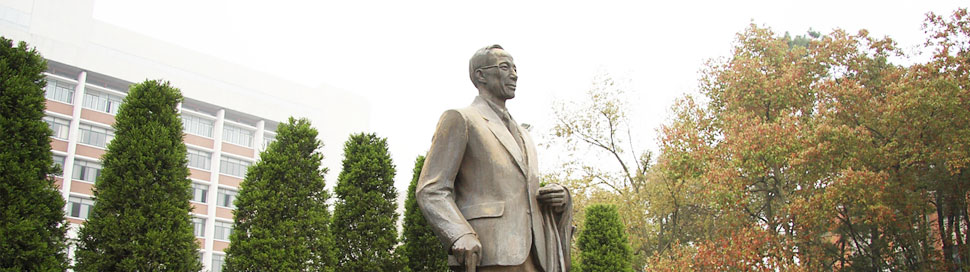
\includegraphics[width=\textwidth]{images/zhukezhen.jpg}}
\institute{College of Computer Science and Technology,  Zhejiang University}


\keywords{Gem5, Linux Kernel, Cross-compiling}
\logo{
\includegraphics[width=2.0cm,height=2.0cm]{images/ZJU.jpg}}

\date{}

\AtBeginSection[]{ 	% 在每个Section前加入Outline Frame
	\frame<handout:0>{
		\frametitle{Outline}
		\tableofcontents[current, currentsubsection]
	}
}


\usetheme{Warsaw}	% Bergen 有点意思	Berkeley	小清新,还不错 Berlin也不错 Copenhagen	Warsaw

%\useoutertheme{split}
%\useinnertheme{default}
%
%\usecolortheme{seahorse}
\begin{document}

\begin{frame}
\titlepage
\end{frame}

\part{Result}
\begin{frame}
\partpage
\end{frame}
\begin{frame}{Result}
\begin{figure}
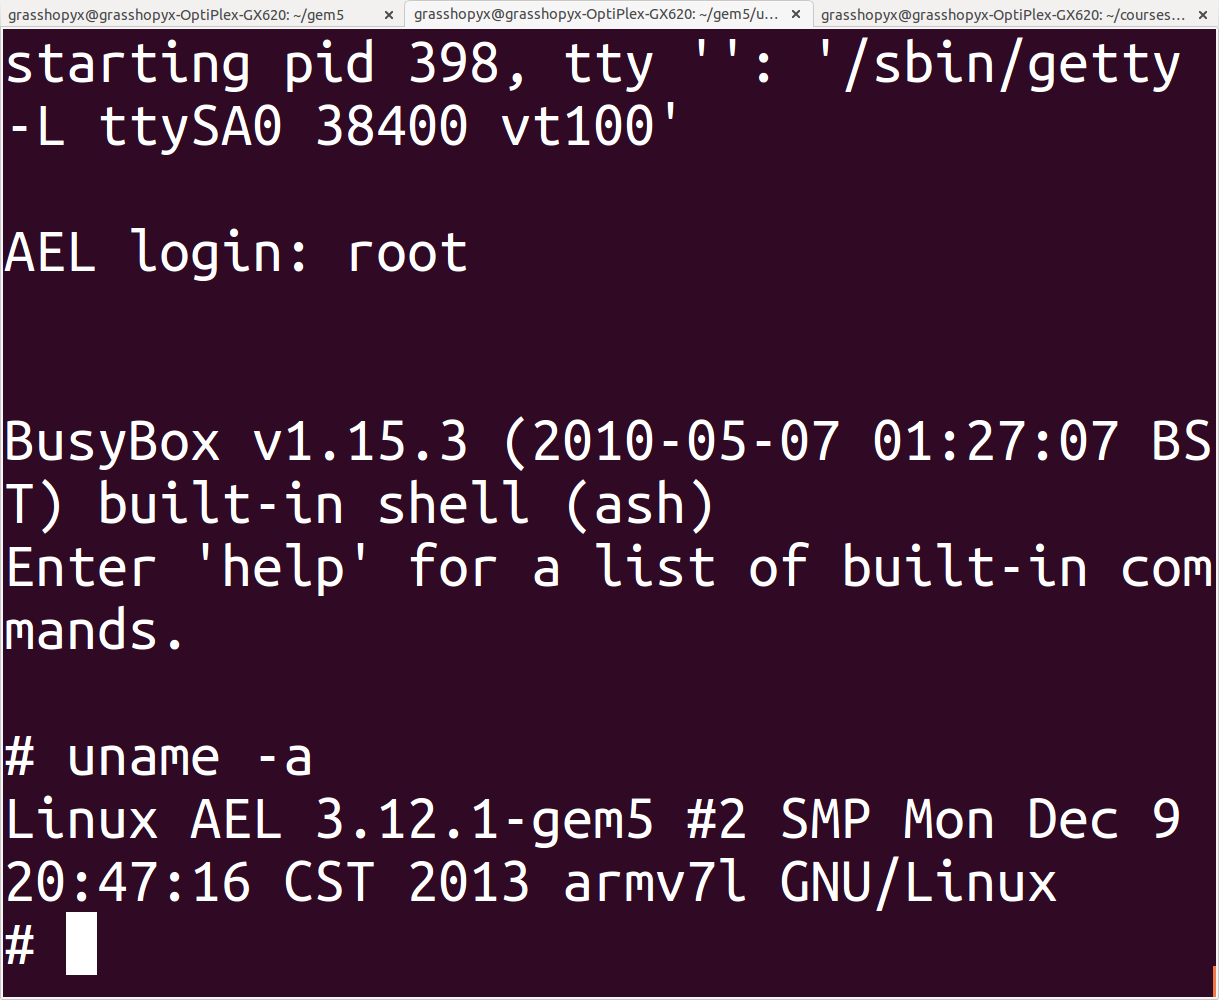
\includegraphics[width=0.7\textwidth]{images/result.png}
\end{figure}
\end{frame}


\part{Introduction}
\begin{frame}
\partpage
\end{frame}

\section{Overview}
\begin{frame}{\secname}
\begin{figure}
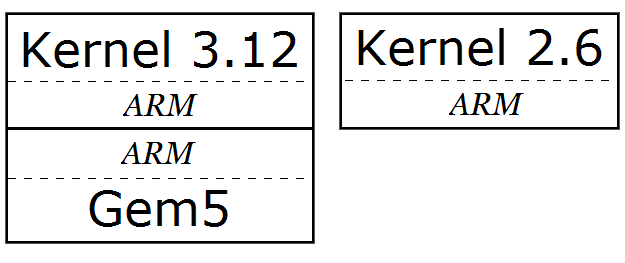
\includegraphics[width=\textwidth]{images/arch2.png}

\end{figure}

\end{frame}

\section{Steps}
\begin{frame}{\secname}
\begin{enumerate}[<alert@+>]
\item
Install requisite packages
\item
Download Gem5 and compile it for ARM --> gem5.opt
\item
Download Linux kernel and cross-compile it for ARM --> vmlinux-3.12
\item
Configure M5\_DIR (vmlinux-3.12, linux-arm-ael.img)
\item
Run and test (m5term)
\end{enumerate}
\end{frame}
\section{Environment}
\begin{frame}{\secname}
\begin{table}
	\caption{Hardware and operating system}
	\begin{tabular}{c|cc}
		\Xhline{2pt}
		Device	&	\multicolumn{2}{c}{Optiplex GX620}\\
		\Xhline{1pt}
				&	CPU				&	Pentium D 3.00GHz X 2	\\
				&	Memory			&	2GB\\
		\Xhline{1.5pt}
		OS		&	\multicolumn{2}{c}{Ubuntu 13.04} \\
		\Xhline{1pt}
				&	ISA				&	AMD64\\
				&	Swap			&	2GB\\
		\Xhline{2pt}
	\end{tabular}
\end{table}
\end{frame}

\part{Obstacles}
\begin{frame}
\partpage
\end{frame}
\section{Compiling failed}
\begin{frame}{\secname}{Gem5}
\begin{block}{Gem5}
\begin{enumerate}[<+- | alert@+>]
\item
Badminton and pingpong time
\item
Inadequate DRAM
\item
scons /build/ARM/gem5.opt -j2
\end{enumerate}
\end{block}
\end{frame}
\begin{frame}{\secname}{Kernel}
\begin{block}{Kernel}
\begin{enumerate}[<+-|alert@+>]
\item
Badminton and pingpong time
\item
make ARCH=arm O=PATH menuconfig
\item
make ARCH=arm CROSS\_COMPILE=arm-linux-gnueabi- O=PATH vmlinux-3.12
\item
Prerequisite
\end{enumerate}
\end{block}
\end{frame}
\section{Running failed}
\begin{frame}{\secname}
\begin{block}{Gem5}
SE mode runs smoothly.\pause
\end{block}
\begin{block}{Kernel on Gem5}
\begin{enumerate}[<+-|alert@+>]
\item
--mem-size
\item
--kernel
\item
--disk-image
\end{enumerate}
\end{block}
\end{frame}

\part{Solution}
\begin{frame}
\partpage
\end{frame}
\begin{frame}{Solution}
\begin{itemize}
\item
Classification: Documentation and videos
\item
Index: Google
\end{itemize}


\end{frame}

\part{Cooperation}
\begin{frame}
\partpage
\end{frame}
\begin{frame}{Cooperation}
\begin{itemize}
\item No divide-and-conquering
\item Discussing
\end{itemize}
\end{frame}

\part{Acknowledgements}
\begin{frame}
\partpage
\end{frame}
\begin{frame}{Acknowledgements}
\begin{itemize}
\item
陈文智
\item
卢忠勇
\item
谢斌、叶敏娇
\item
Mark Chen, zxz and etc.
\end{itemize}
\end{frame}


%\begin{frame}
%\partpage
%\end{frame}
%\begin{frame}{古中国数学}{定理发现}
%中国在3000多年前就知道勾股数的概念,比古希腊更早一些。
%《周髀算经》的记载:
%\begin{itemize}
%\item 公元前11世纪,商高答周公问:
%\begin{quote}
%勾广三,股修四,径隅五。
%\end{quote}
%\item 又载公元前7--6世纪陈子荣答方问,表述了勾股定理的一般形式:
%\begin{quote}
%若求邪至日者,以日下为勾,日高为股,勾股各自乘,并而开方除之,得邪至日。
%\end{quote}
%\end{itemize}
%
%\end{frame}

\newpage
\end{document}